\section{Electromagnetism}

\begin{multicols}{2}


\subsection[Induced Magnetic Field from a Coil]{Induced Magnetic Field from \hfill \\ a Coil}

\begin{center}
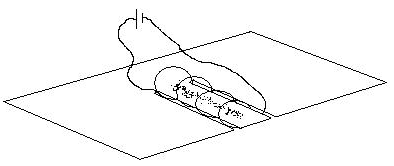
\includegraphics[width=0.45\textwidth]{./img/induced-mag-field-coil.png}
\end{center}

\begin{description*}
%\item[Subtopic:]{}
\item[Materials:]{Dry cell, 50 cm of wire, cardboard, iron wool}
%\item[Setup:]{}
\item[Procedure:]{Coil a wire through a piece of cardboard and connect to a dry cell. Use the iron wool to sprinkle iron filings inside the coil and around either end.}
%\item[Hazards:]{}
%\item[Questions:]{}
\item[Observations:]{The filings create a single solid line the length of the coil, spreading out at each end.}
\item[Theory:]{A coil of wire creates a single strong magnetic field inside it in one direction. At the poles, the field spreads out again. The Right Hand Rule can be used to find the direction of the field.}
%\item[Applications:]{}
%\item[Notes:]{}
\end{description*}

\subsection[Induced Magnetic Field from a Wire]{Induced Magnetic Field from \hfill \\ a Wire}

\begin{center}
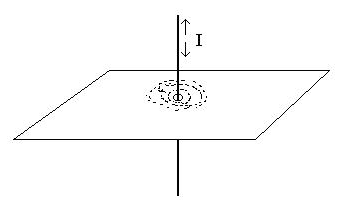
\includegraphics[width=0.45\textwidth]{./img/induced-mag-field-wire.png}
\end{center}

\begin{description*}
%\item[Subtopic:]{}
\item[Materials:]{Dry cell, straight wire, paper, iron wool}
%\item[Setup:]{}
\item[Procedure:]{Cut a hole in the paper so that the wire passes vertically through the middle and the paper lies flat. Connect the wire to the dry cell. Sprinkle iron filings across the paper.}
%\item[Hazards:]{}
%\item[Questions:]{}
\item[Observations:]{The filings form concentric circles around the wire.}
\item[Theory:]{Current in a straight wire produces a magnetic field around the wire in concentric circles. The filings align themselves in the field to show the lines of force. the Right Hand Rule can be used to find the direction of the field.}
%\item[Applications:]{}
%\item[Notes:]{}
\end{description*}

\subsection{Making a Galvanometer}

\begin{center}
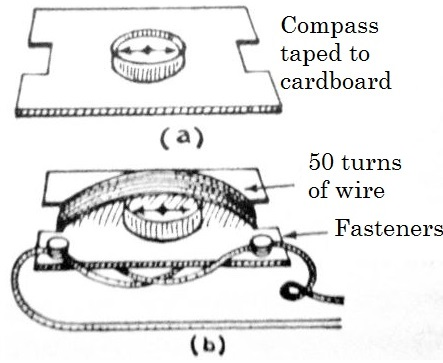
\includegraphics[width=0.4\textwidth]{./img/galvanometer.jpg}
\end{center}

\begin{description*}
%\item[Subtopic:]{}
\item[Materials:]{Cardboard, tape, compass, copper wire, fasteners/thumb pins}
\item[Setup:]{Tape the compass to the cardboard and wind 50 turns of wire around it, leaving about 50 cm free at each end. Fix the wire using fasteners. Scrape the insulation at the free ends of the wire.}
\item[Procedure:]{Connect to a dry cell. Still watching the compass, reverse the terminals of the wires.}
%\item[Hazards:]{}
%\item[Questions:]{}
%\item[Observations:]{}
\item[Theory:]{The compass deflects, revealing the presence of electric current. Reversing the connection changes the direction of current and thus magnetic field.}
%\item[Applications:]{}
%\item[Notes:]{}
\end{description*}

%\subsection{Construction of a Galvanometer} % Move elsewhere??
%
%%\begin{center}
%%\includegraphics[width=0.4\textwidth]{./img/source/.png}
%%\end{center}
%
%\begin{description*}
%%\item[Subtopic:]{}
%\item[Materials:]{Magnet, pin/needle, coated copper wire or speaker wire, dry cells, water, empty water bottle, small piece of paper, knife, connecting wires, cello tape}
%\item[Setup:]{Cut the bottom 3 cm of a water bottle to make a shallow dish. Magnetize the needle by rubbing it several times in one direction with a magnet. Coil the wire around the dish about 20 times and secure with cello tape. Use a knife to scrape about 2 cm of the coating off of each end of the wire. Fill the dish half way with water. Stitch the pin into a small piece of paper so that the pin is secure against one side.}
%\item[Procedure:]{ Place the pin and paper gently onto the surface of the water in the dish so it floats. Use connecting wires to connect the dry cells to both ends of the coiled wire. Observe the reaction of the needle.}
%%\item[Hazards:]{}
%%\item[Questions:]{}
%\item[Observations:]{The pin rests in the N-S direction. After connecting the dry cells, the pin deflects.}
%\item[Theory:]{The pin deflects because the magnetic field produced by the coil is stronger than the earth's field. The galvanometer detects whenever there is the flow of current in the wire.}
%\item[Applications:]{}
%%\item[Notes:]{}
%\end{description*}

\subsection{Spinning Compass}

\begin{center}
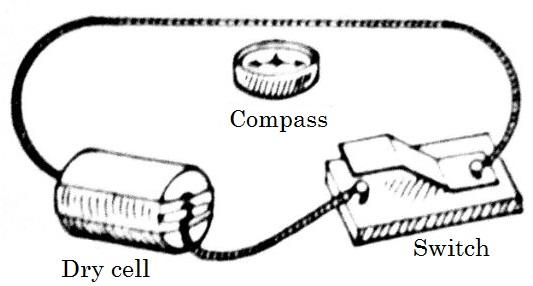
\includegraphics[width=0.38\textwidth]{./img/spinning-compass.jpg}
\end{center}

\begin{description*}
%\item[Subtopic:]{}
\item[Materials:]{Power source, wire, compass/magnetized pin}
%\item[Setup:]{}
\item[Procedure:]{Connect the wire to the power supply. Run the wire over the compass in a straight line.}
%\item[Hazards:]{}
%\item[Questions:]{}
\item[Observations:]{If the current is DC, the compass will turn to face a new direction. If AC, the compass will spin back and forth quickly.}
\item[Theory:]{Current in a straight wire creates a magnetic field around the wire. DC current produces a steady magnetic field in one direction (circular), so the magnet aligns itself with the field. AC current produces a constantly shifting field, so the compass will spin, trying to align itself as the field changes direction.}
%\item[Applications:]{}
%\item[Notes:]{}
\end{description*}

\subsection{Force on a Current-Carrying Conductor in a Magnetic Field}

\begin{center}
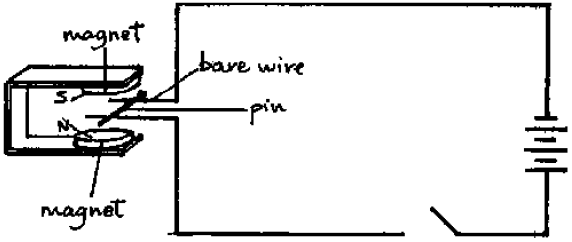
\includegraphics[width=0.49\textwidth]{./img/source/force-wire.png}
\end{center}

\begin{description*}
%\item[Subtopic:]{}
\item[Materials:]{Dry cells, pin, 2 speaker magnets, wire, switch}
%\item[Setup:]{}
\item[Procedure:]{Connect the circuit as shown and place a pin across the straight bare wires between the poles of the magnets and close the switch \emph{for a short time only}.}
%\item[Hazards:]{}
%\item[Questions:]{}
\item[Observations:]{The pin rolls along the straight wires.}
\item[Theory:]{The pin closes the circuit and thus has current running through it. The magnetic field around the pin produces a force on the current in the pin, causing it to roll.}
\item[Applications:]{Electric motors, loudspeakers}
%\item[Notes:]{}
\end{description*}

%==================================================================================================%

\section*{Electromagnetic Induction}


\subsection{Creating Current in a Wire} % PIC!!

%\begin{center}
%\includegraphics[width=0.4\textwidth]{./img/source/.png}
%\end{center}

\begin{description*}
%\item[Subtopic:]{}
\item[Materials:]{50 cm of wire, ammeter or bulb, strong magnet}
%\item[Setup:]{}
\item[Procedure:]{Coil the wire to make a solenoid, connecting the free ends to an ammeter or bulb. Use a bar magnet and pass it through the solenoid.}
%\item[Hazards:]{}
%\item[Questions:]{}
\item[Observations:]{As the magnet passes through the coil, the ammeter or bulb shows a current. When the magnet stops moving or leaves the coil, the current ceases.}
\item[Theory:]{A magnetic field moving perpendicular to a conductor induces a current in the conductor. The current strength can be increased by increasing the number of coils or by using a stronger magnet.}
%\item[Applications:]{}
%\item[Notes:]{}
\end{description*}

\subsection{Creating Alternating Current}

%\begin{center}
%\includegraphics[width=0.4\textwidth]{./img/.png}
%\end{center}

\begin{description*}
%\item[Subtopic:]{}
\item[Materials:]{Syringe, 50 cm of wire, strong bar magnet, ammeter/bulb, small piece of cloth}
%\item[Setup:]{}
\item[Procedure:]{Wrap the wire around a syringe multiple times and connect the ends to an ammeter or bulb. Place a small wad of cloth in the bottom of the syringe and insert the magnet. Cover the opening with your thumb and shake. The cloth and your thumb protect the magnet as it bounces back and forth, creating an alternating current in the coil.}
%\item[Hazards:]{}
%\item[Questions:]{}
%\item[Observations:]{}
%\item[Theory:]{}
%\item[Applications:]{}
%\item[Notes:]{}
\end{description*}

\columnbreak

%==================================================================================================%

\section*{Generators}


\subsection{Simple Motor}

\begin{center}
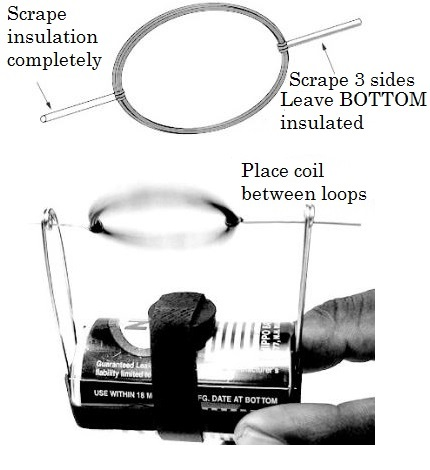
\includegraphics[width=0.49\textwidth]{./img/simple-motor-final.jpg}
\end{center}

\begin{description*}
%\item[Subtopic:]{}
\item[Materials:]{Dry cell, insulated copper wire (1~m), 2 paper clips/safety pins, rubber bands, speaker magnet}
\item[Setup:]{Make several turns of copper wire around the dry cell, leaving about 5 cm on either side. Use a knife to remove the insulation from all sides of the wire on one end, and 3 sides on the other end. Bend two paper clips as shown to make supports for the wire or use safety pins.}
\item[Procedure:]{Attach the paper clips/safety pins to either end of the dry cell using a rubber band. Lay the copper wire coil across the paper clip holders. Bring the coil close to a speaker magnet.}
%\item[Hazards:]{}
%\item[Questions:]{}
\item[Observations:]{The coil begins to turn when brought close to the magnet.}
\item[Theory:]{The magnetic field applies a force to the current-carrying wire following Fleming's left-hand rule and causes the loop to spin. If the current is increased the coil spins faster, showing the force is proportional to the current. If the current is reversed the coil will rotate in the other direction. If there is a stronger magnet the coil spins faster, which shows the force is proportional to the magnetic field strength. If all of the insulation is scratched off from both sides then the loop will not spin but will instead reach an equilibrium position where the force acting on the top and bottom of the loop are balanced.}
%\item[Applications:]{}
%\item[Notes:]{}
\end{description*}

\columnbreak

\subsection{Wind Turbine}
\label{sub:wind-turbine}

\begin{center}
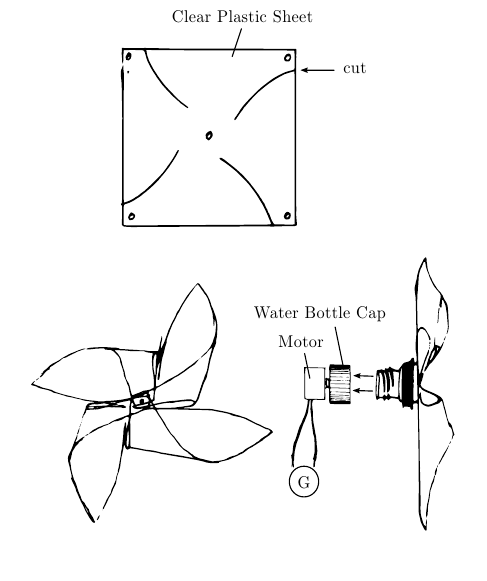
\includegraphics[width=0.49\textwidth]{./img/wind-turbine.png}
\end{center}

\begin{description*}
%\item[Subtopic:]{}
\item[Materials:]{30 cm $\times$ 30 cm flexible plastic sheet, pin, scissors, super glue, plastic water bottle, small motor (e.g. from car stereo), connecting wires, galvanometer}
\item[Propeller:]{Make 5 small holes in the plastic sheet - one at each corner and one in the middle. Cut along the curved lines shown. Fold each corner towards the centre so that all five holes are aligned and glue them in place. Cut the top off of a water bottle just below the lip where the cap sits. Glue the bottle top to the propeller as shown. }
\item[Generator:]{Make a small hole in the centre of the bottle cap using a pin. Glue the top of the cap to the motor wheel so that the two spin together evenly.}
\item[Setup:]{Screw the propeller onto the generator like closing a bottle. The propeller should be able to turn freely on the motor. Connect the terminals of the motor to the terminals of the galvanometer.}
\item[Procedure:]{Hold the propeller upright into the wind so that it spins.}
%\item[Hazards:]{}
%\item[Questions:]{}
\item[Observations:]{The galvanometer will deflect to show that a current is being created in the wire.}
\item[Theory:]{Mechanical energy (wind) is converted into electrical energy (electric current) using a generator. The generator uses a magnet and motion to produce an electric current.}
\item[Applications:]{Sustainable energy sources}
%\item[Notes:]{}
\end{description*}

\columnbreak

\subsection{Water Turbine}
\label{sub:water-turbine}

\begin{center}
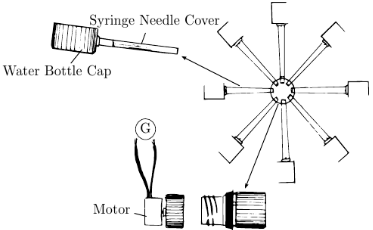
\includegraphics[width=0.49\textwidth]{./img/water-turbine.png}
\end{center}

\begin{description*}
%\item[Subtopic:]{}
\item[Materials:]{Plastic bottle, small motor (e.g. from car stereo), super glue, \nameref{sec:heatsources}, heated nail or soldering iron, 9 water bottle caps, 8 syringe needle caps, scissors, water and pitcher, connecting wires, galvanometer}
\item[Water Wheel:]{Using a hot nail or soldering iron, melt the open end of a syringe needle cap to the side of a water bottle cap to create a sort of spoon. Repeat 7 more times for a total of 8 pieces. Cut the top off a water bottle just below the lip which holds the cap. Melt a plastic cap over the cut end of the bottle top so that the threaded side is open. Use the hot nail or soldering iron to melt 8 holes evenly around the side of this central bottle cap. Insert the 8 spokes into the holes so that they create an 8-spoke wheel with all of the cups facing in one direction at equal distances from the centre. Melt the plastic around each spoke to secure them in place.}
\item[Generator:]{Make a small hole in the centre of the bottle cap using a pin. Glue the top of the cap to the motor wheel so that the two spin together evenly.}
\item[Setup:]{Screw the water wheel onto the generator like closing a bottle. The water wheel should be able to turn freely on the motor. Connect the terminals of the motor to the terminals of the galvanometer.}
\item[Procedure:]{Pour water from a pitcher or spout and place the water wheel under the water so that it turns vertically.}
%\item[Hazards:]{}
%\item[Questions:]{}
\item[Observations:]{The galvanometer will deflect to show that a current is being created in the wire.}
\item[Theory:]{Mechanical energy (falling water and subsequent rotating water wheel) is converted into electrical energy (electric current) using a generator. The generator uses a magnet and motion to produce an electric current.}
\item[Applications:]{Sustainable energy sources}
%\item[Notes:]{}
\end{description*}

\end{multicols}

\subsection{Inverter: Converting DC to AC} \label{sub:inverter}

\begin{center}
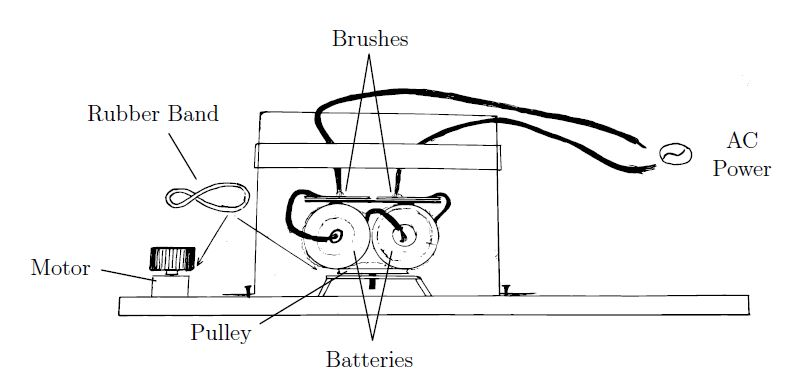
\includegraphics[width=0.8\textwidth]{./img/inverter-2.jpg}
%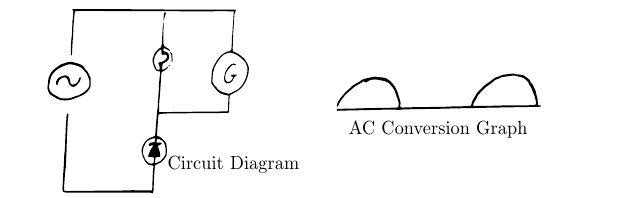
\includegraphics[width=0.4\textwidth]{./img/half-wave-rectifier.png}
%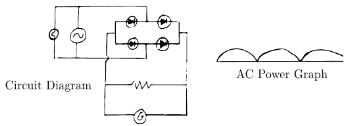
\includegraphics[width=0.4\textwidth]{./img/full-wave-rectifier.png}
\end{center}

\begin{multicols}{2}

\begin{description*}
%\item[Subtopic:]{}
\item[Materials:]{4 dry cells, aluminum outer coating of dead dry cell, thin cardboard, super glue, soldering iron and flux, several small nails, connecting wires, board at least 30 cm long, bulb or galvanometer, scissors, knife, retort stand, small motor, horizontal pulley, rubber band, pliers, multimeter}
\item[Setup:]{Attach the pulley and motor near one end of the board so that they are free to rotate horizontally as shown. Connect the pulley and motor using a rubber band so that they rotate together. Solder a connecting wire from the positive terminal of one dry cell to the negative terminal of another so that they are connected in series but still packaged together side-by-side. Glue the battery pack on its side to the centre of the horizontal pulley. 

Glue a small 5 cm square piece of cardboard on top of the battery pack. Mark the centre of rotation of the pulley and battery pack system on the cardboard. Take a piece of aluminum from a dead dry cell and break it into 2 equal pieces (5 cm $\times$ 3 cm) using pliers. Glue the pieces to the cardboard leaving a small space between them so that the hole marking the centre of rotation can be seen. Solder or glue a short connecting wire from the free end of one battery to one of the aluminum plates. Repeat for the other battery and aluminum plate. Check connections using a multimeter. 

Cut a piece of cardboard 10 cm $\times$ 4 cm and fold it in half the long way. Cut two very small holes in the center of the folded edge about 2 cm apart. Insert connecting wires into each hole so that they stick out about 2 cm. Remove the insulation from the wires so that the copper ends form brush shapes and are free to bend slightly. Extend the connecting wires to a bulb or galvanometer and solder or glue the ends to the terminals.

Check the circuit using a multimeter and 2 dry cells across the brush ends. Suspend the bulb/brush circuit about the rotating metal plates so that the wire brushes just touch the metal plates. If each brush is touching a different metal plate, the bulb or galvanometer should indicate a current.}
\item[Procedure:]{Touch the wire brushes to opposite plates to show that a direct current is flowing and the bulb/galvanometer shows a single direction of current. Switch the plates that the brushes are touching to show that, again a direct current is flowing in the opposite direction as before. Connect the motor to the batteries so that the system rotates under the brushes.}
%\item[Hazards:]{}
%\item[Questions:]{}
\item[Observations:]{When the metal plates are rotating under the brushes, the galvanometer changes direction quickly. The behaviour of the galvanometer/bulb is different depending on whether the plates are rotating.}
\item[Theory:]{The galvanometer changes direction because the direction of current is changing every time the plates switch brushes. The system is converting direct current (DC) of the battery pack to alternating current (AC) in the bulb or galvanometer.}
%\item[Applications:]{}
\item[Notes:]{Normally, alternating current changes direction 80 times per second, which we cannot see with our eyes. Therefore, the difference between AC and DC is not visible in a normal household or school electrical system. In order to see the effect of AC, we need to slow down the frequency to the point where we can see the direction changing in the galvanometer or bulb.}
\end{description*}

\end{multicols}

%==================================================================================================%




\pagebreak
